% Created 2023-07-24 Mon 16:34
% Intended LaTeX compiler: pdflatex
\documentclass[11pt]{article}
\usepackage[utf8]{inputenc}
\usepackage[T1]{fontenc}
\usepackage{graphicx}
\usepackage{longtable}
\usepackage{wrapfig}
\usepackage{rotating}
\usepackage[normalem]{ulem}
\usepackage{amsmath}
\usepackage{amssymb}
\usepackage{capt-of}
\usepackage{hyperref}
\usepackage{minted}
\usepackage[a4paper]{geometry}
\usepackage{mathtools}
\author{Alexander Huss}
\date{\today}
\title{The Drell--Yan process: \(\mathrm{p}\mathrm{p} \to \ell^+\ell^-\)}
\hypersetup{
 pdfauthor={Alexander Huss},
 pdftitle={The Drell--Yan process: \(\mathrm{p}\mathrm{p} \to \ell^+\ell^-\)},
 pdfkeywords={},
 pdfsubject={},
 pdfcreator={Emacs 28.2 (Org mode 9.7)}, 
 pdflang={English}}
\begin{document}

\maketitle
\tableofcontents



\section{Introduction}
\label{sec:orga7871c1}
We will implement the process \(\mathrm{p}\mathrm{p} \to \ell^+\ell^-\).
This gives us access to a simple hadron-collider process that constitutes a ``Standard Candle'' at the LHC and has a wide range of applications.

\section{Cross section}
\label{sec:orgef4c443}

\subsection{Partonic cross section}
\label{sec:orgc9f1564}

The squared Matrix Element is essentially the same as the one we looked at in the \(\mathrm{e}^+\mathrm{e}^- \to \mu^+ \mu^-\) case.
To make life a little easier for us, we integrated out the kinematics of the \(\mathrm{Z}/\gamma^*\to\ell^+\ell^-\) system.
In particular, this means that we're no longer sensitive to the \(G_2\) function in the \(\mathrm{e}^+\mathrm{e}^-\) case that was parity odd.

We begin by defining separate \emph{lepton} and \emph{hadron} structure functions
\begin{align}
  L_{\gamma\gamma}(\hat{s})
  &=
  \frac{2}{3}\;\frac{\alpha\; Q_\ell^2}{\hat{s}}
  \\
  L_{\mathrm{Z}\mathrm{Z}}(\hat{s})
  &=
  \frac{2}{3}\;\frac{\alpha\; (v_\ell^2 + a_\ell^2)}{\hat{s}}\;
  \biggl\lvert\frac{\hat{s}}{\hat{s} - M_\mathrm{Z}^2 + \mathrm{i}\Gamma_\mathrm{Z}M_\mathrm{Z}}\biggr\rvert^2
  \\
  L_{\mathrm{Z}\gamma}(\hat{s})
  &=
  \frac{2}{3}\;\frac{\alpha\; v_\ell Q_\ell }{\hat{s}}\;
  \frac{\hat{s}}{\hat{s} - M_\mathrm{Z}^2 + \mathrm{i}\Gamma_\mathrm{Z}M_\mathrm{Z}}
\end{align}
and (\(N_c = 3\))
\begin{align}
  \mathcal{H}^{(0)}_{\gamma\gamma}(\hat{s})
  &=
  16\pi\,N_c \, \alpha\;\hat{s} \; Q_q^2
  \\
  \mathcal{H}^{(0)}_{\mathrm{Z}\mathrm{Z}}(\hat{s})
  &=
  16\pi\,N_c \, \alpha\;\hat{s} \; (v_q^2 + a_q^2)
  \\
  \mathcal{H}^{(0)}_{\mathrm{Z}\gamma}(\hat{s})
  &=
  16\pi\,N_c \, \alpha\;\hat{s} \; v_q Q_q
\end{align}
that we can use to assemble the \emph{partonic} cross section:
\begin{align}
  \hat{\sigma}_{\bar{q}q\to\ell^+\ell^-}(p_a,\,p_b)
  &=
  \frac{1}{2\hat{s}} \; \frac{1}{36} \; \biggl\{
  L_{\gamma\gamma}(\hat{s}) \mathcal{H}^{(0)}_{\gamma\gamma}(\hat{s})
  + L_{\mathrm{Z}\mathrm{Z}}(\hat{s}) \mathcal{H}^{(0)}_{\mathrm{Z}\mathrm{Z}}(\hat{s})
  + 2\mathrm{Re}\Bigl[ L_{\mathrm{Z}\gamma}(\hat{s}) \mathcal{H}^{(0)}_{\mathrm{Z}\gamma}(\hat{s}) \Bigr]
  \biggr\}
\end{align}

\subsubsection{Implementation}
\label{sec:orgafc8e42}
We'll use a simple class to save and retrieve Standard Model parameters including some convenience functions.
We next implement the different structure functions (we need the additional quark id \texttt{qid} to distinguish up-type from down-type quarks as they have different couplings to the Z boson.
\begin{minted}[frame=lines,fontsize=\scriptsize]{python}
def L_yy(shat: float, par=PARAM) -> float:
    return (2./3) * (par.alpha/shat) * par.Ql**2
def L_ZZ(shat: float, par=PARAM) -> float:
    return (2./3.) * (par.alpha/shat) * (par.vl**2+par.al**2) * abs(par.propZ(shat))**2
def L_Zy(shat: float, par=PARAM) -> float:
    return (2./3.) * (par.alpha/shat) * par.vl*par.Ql * par.propZ(shat).real
def H0_yy(shat: float, qid: int, par=PARAM) -> float:
    return 16.*math.pi * 3. * par.alpha*shat * par.Qq(qid)**2
def H0_ZZ(shat: float, qid: int, par=PARAM) -> float:
    return 16.*math.pi * 3. * par.alpha*shat * (par.vq(qid)**2+par.aq(qid)**2)
def H0_Zy(shat: float, qid: int, par=PARAM) -> float:
    return 16.*math.pi * 3. * par.alpha*shat * par.vq(qid)*par.Qq(qid)
\end{minted}
We can now use those structure functions to implement the partonic cross section
\begin{minted}[frame=lines,fontsize=\scriptsize]{python}
def cross_partonic(shat: float, qid: int, par=PARAM) -> float:
    return (1./2./shat) * (1./36.) * (
            L_yy(shat, par) * H0_yy(shat, qid, par)
        +   L_ZZ(shat, par) * H0_ZZ(shat, qid, par)
        +2.*L_Zy(shat, par) * H0_Zy(shat, qid, par)
    )
\end{minted}

\subsection{Hadronic cross section and lepton-pair observables}
\label{sec:org77471b1}
The hadronic cross section is obtained by convoluting the partonic one with the parton distribution functions:
\begin{align}
  \sigma_{A B \to \ell^+\ell^-} (P_A, P_B)
  &=
  \sum_{a,b}
  \int_0^1\mathrm{d}x_a \; f_{a\vert A}(x_a)
  \int_0^1\mathrm{d}x_b \; f_{b\vert B}(x_b) \;
  \hat{\sigma}_{ab\to\ell^+\ell^-}(x_a P_A,\,x_b P_B)
  \,,
\end{align}
where the indices \(a\) and \(b\) run over all possible partons inside the hadrons \(A\) and \(B\), respectively.
In the case of the Drell--Yan process at lowest order, the two possible ``channels'' are:  \((a,b) \in \{(q,\bar{q}),\,(\bar{q},q)\}\).

We have already integrated out the lepton decay kinematics but have still access to the information of the intermediate gauge boson, \(q^\mu = (p_a+p_b)^\mu = (x_a P_A + x_b P_B)^\mu\).
To get the differential cross section, we need to differentiate the above formula, which amounts to injecting delta distributions for the observables we're after.
Two variables suitable are the invariant mass, \(M_{\ell\ell} = \sqrt{q^2}\), and the rapidity, \(Y_{\ell\ell} = \tfrac{1}{2}\ln\Bigl(\tfrac{q^0+q^3}{q^0-q^3}\Bigr)\), of the di-lepton system.
Being differential in these two observables, we're left with no more integrations at LO and the entire kinematics is fixed:
\begin{align}
  \frac{\mathrm{d}^2\sigma_{A B \to \ell^+\ell^-}}{\mathrm{d}M_{\ell\ell}\mathrm{d}Y_{\ell\ell}}
  &=
  f_{a\vert A}(x_a) \; f_{b\vert B}(x_b) \; \frac{2\,M_{\ell\ell}}{E_\mathrm{cm}^2} \;
  \hat{\sigma}_{ab\to\ell^+\ell^-l}(x_a P_A,\,x_b P_B)
  \;\bigg\vert_{x_{a/b}\equiv\tfrac{M_{\ell\ell}}{E_\mathrm{cm}}\mathrm{e}^{\pm Y_{\ell\ell}}}
\end{align}

\subsubsection{Implementation}
\label{sec:org7397e88}
Let's implement the hadronic differential cross section
\begin{minted}[frame=lines,fontsize=\scriptsize]{python}
def diff_cross(Ecm: float, Mll: float, Yll: float, par=PARAM) -> float:
    xa = (Mll/Ecm) * math.exp(+Yll)
    xb = (Mll/Ecm) * math.exp(-Yll)
    s = Ecm**2
    shat = xa*xb*s
    lum_dn = (
          par.pdf.xfxQ(+1, xa, Mll) * par.pdf.xfxQ(-1, xb, Mll)  # (d,dbar)
        + par.pdf.xfxQ(+3, xa, Mll) * par.pdf.xfxQ(-3, xb, Mll)  # (s,sbar)
        + par.pdf.xfxQ(+5, xa, Mll) * par.pdf.xfxQ(-5, xb, Mll)  # (b,bbar)
        + par.pdf.xfxQ(-1, xa, Mll) * par.pdf.xfxQ(+1, xb, Mll)  # (dbar,d)
        + par.pdf.xfxQ(-3, xa, Mll) * par.pdf.xfxQ(+3, xb, Mll)  # (sbar,s)
        + par.pdf.xfxQ(-5, xa, Mll) * par.pdf.xfxQ(+5, xb, Mll)  # (bbar,b)
        ) / (xa*xb)
    lum_up = (
          par.pdf.xfxQ(+2, xa, Mll) * par.pdf.xfxQ(-2, xb, Mll)  # (u,ubar)
        + par.pdf.xfxQ(+4, xa, Mll) * par.pdf.xfxQ(-4, xb, Mll)  # (c,cbar)
        + par.pdf.xfxQ(-2, xa, Mll) * par.pdf.xfxQ(+2, xb, Mll)  # (ubar,u)
        + par.pdf.xfxQ(-4, xa, Mll) * par.pdf.xfxQ(+4, xb, Mll)  # (cbar,c)
        ) / (xa*xb)
    return par.GeVpb * (2.*Mll/Ecm**2) * (
         lum_dn * cross_partonic(shat, 1, par)
        +lum_up * cross_partonic(shat, 2, par)
        )
\end{minted}



\section{Playground}
\label{sec:org0694658}

\subsection{Export source code}
\label{sec:org23ae6f9}
We can export the python source code to a file \texttt{main.py}:
\begin{minted}[frame=lines,fontsize=\scriptsize]{python}
import lhapdf
import math
import cmath
import numpy as np
import scipy
class Parameters(object):
    """very simple class to manage Standard Model Parameters"""

    #> conversion factor from GeV^{-2} into picobarns [pb]
    GeVpb = 0.3893793656e9

    def __init__(self, **kwargs):
        #> these are the independent variables we chose:
        #>  *  sw2 = sin^2(theta_w) with the weak mixing angle theta_w
        #>  *  (MZ, GZ) = mass & width of Z-boson
        self.sw2  = kwargs.pop("sw2", 0.22289722252391824808)
        self.MZ   = kwargs.pop("MZ", 91.1876)
        self.GZ   = kwargs.pop("GZ", 2.495)
        self.sPDF = kwargs.pop("sPDF", "NNPDF31_nnlo_as_0118_luxqed")
        self.iPDF = kwargs.pop("iPDF", 0)
        if len(kwargs) > 0:
            raise RuntimeError("passed unknown parameters: {}".format(kwargs))
        #> we'll cache the PDF set for performance
        lhapdf.setVerbosity(0)
        self.pdf = lhapdf.mkPDF(self.sPDF, self.iPDF)
        #> let's store some more constants (l, u, d = lepton, up-quark, down-quark)
        self.Ql = -1.;    self.I3l = -1./2.;  # charge & weak isospin
        self.Qu = +2./3.; self.I3u = +1./2.;
        self.Qd = -1./3.; self.I3d = -1./2.;
        self.alpha = 1./132.2332297912836907
        #> and some derived quantities
        self.sw = math.sqrt(self.sw2)
        self.cw2 = 1.-self.sw2  # cos^2 = 1-sin^2
        self.cw = math.sqrt(self.cw2)
    #> vector & axial-vector couplings to Z-boson
    @property
    def vl(self) -> float:
        return (self.I3l-2*self.Ql*self.sw2)/(2.*self.sw*self.cw)
    @property
    def al(self) -> float:
        return self.I3l/(2.*self.sw*self.cw)
    def vq(self, qid: int) -> float:
        if qid == 1:  # down-type
            return (self.I3d-2*self.Qd*self.sw2)/(2.*self.sw*self.cw)
        if qid == 2:  # up-type
            return (self.I3u-2*self.Qu*self.sw2)/(2.*self.sw*self.cw)
        raise RuntimeError("vq called with invalid qid: {}".format(qid))
    def aq(self, qid: int) -> float:
        if qid == 1:  # down-type
            return self.I3d/(2.*self.sw*self.cw)
        if qid == 2:  # up-type
            return self.I3u/(2.*self.sw*self.cw)
        raise RuntimeError("aq called with invalid qid: {}".format(qid))
    def Qq(self, qid: int) -> float:
        if qid == 1:  # down-type
            return self.Qd
        if qid == 2:  # up-type
            return self.Qu
        raise RuntimeError("Qq called with invalid qid: {}".format(qid))
    #> the Z-boson propagator
    def propZ(self, s: float) -> complex:
        return s/(s-complex(self.MZ**2,self.GZ*self.MZ))
#> we immediately instantiate an object (default values) in global scope
PARAM = Parameters()

def L_yy(shat: float, par=PARAM) -> float:
    return (2./3) * (par.alpha/shat) * par.Ql**2
def L_ZZ(shat: float, par=PARAM) -> float:
    return (2./3.) * (par.alpha/shat) * (par.vl**2+par.al**2) * abs(par.propZ(shat))**2
def L_Zy(shat: float, par=PARAM) -> float:
    return (2./3.) * (par.alpha/shat) * par.vl*par.Ql * par.propZ(shat).real
def H0_yy(shat: float, qid: int, par=PARAM) -> float:
    return 16.*math.pi * 3. * par.alpha*shat * par.Qq(qid)**2
def H0_ZZ(shat: float, qid: int, par=PARAM) -> float:
    return 16.*math.pi * 3. * par.alpha*shat * (par.vq(qid)**2+par.aq(qid)**2)
def H0_Zy(shat: float, qid: int, par=PARAM) -> float:
    return 16.*math.pi * 3. * par.alpha*shat * par.vq(qid)*par.Qq(qid)
def cross_partonic(shat: float, qid: int, par=PARAM) -> float:
    return (1./2./shat) * (1./36.) * (
            L_yy(shat, par) * H0_yy(shat, qid, par)
        +   L_ZZ(shat, par) * H0_ZZ(shat, qid, par)
        +2.*L_Zy(shat, par) * H0_Zy(shat, qid, par)
    )
def diff_cross(Ecm: float, Mll: float, Yll: float, par=PARAM) -> float:
    xa = (Mll/Ecm) * math.exp(+Yll)
    xb = (Mll/Ecm) * math.exp(-Yll)
    s = Ecm**2
    shat = xa*xb*s
    lum_dn = (
          par.pdf.xfxQ(+1, xa, Mll) * par.pdf.xfxQ(-1, xb, Mll)  # (d,dbar)
        + par.pdf.xfxQ(+3, xa, Mll) * par.pdf.xfxQ(-3, xb, Mll)  # (s,sbar)
        + par.pdf.xfxQ(+5, xa, Mll) * par.pdf.xfxQ(-5, xb, Mll)  # (b,bbar)
        + par.pdf.xfxQ(-1, xa, Mll) * par.pdf.xfxQ(+1, xb, Mll)  # (dbar,d)
        + par.pdf.xfxQ(-3, xa, Mll) * par.pdf.xfxQ(+3, xb, Mll)  # (sbar,s)
        + par.pdf.xfxQ(-5, xa, Mll) * par.pdf.xfxQ(+5, xb, Mll)  # (bbar,b)
        ) / (xa*xb)
    lum_up = (
          par.pdf.xfxQ(+2, xa, Mll) * par.pdf.xfxQ(-2, xb, Mll)  # (u,ubar)
        + par.pdf.xfxQ(+4, xa, Mll) * par.pdf.xfxQ(-4, xb, Mll)  # (c,cbar)
        + par.pdf.xfxQ(-2, xa, Mll) * par.pdf.xfxQ(+2, xb, Mll)  # (ubar,u)
        + par.pdf.xfxQ(-4, xa, Mll) * par.pdf.xfxQ(+4, xb, Mll)  # (cbar,c)
        ) / (xa*xb)
    return par.GeVpb * (2.*Mll/Ecm**2) * (
         lum_dn * cross_partonic(shat, 1, par)
        +lum_up * cross_partonic(shat, 2, par)
        )
if __name__ == "__main__":
    Ecm = 8e3
    for Yll in np.linspace(-3.6, 3.6, 100):
        dsig = scipy.integrate.quad(lambda M: diff_cross(Ecm,M,Yll), 80., 100., epsrel=1e-3)
        print("#Yll {:e} {:e} {:e}".format(Yll,dsig[0],dsig[1]))
    for Mll in np.linspace(10, 200, 200):
        dsig = scipy.integrate.quad(lambda Y: diff_cross(Ecm,Mll,Y), -3.6, +3.6, epsrel=1e-3)
        print("#Mll {:e} {:e} {:e}".format(Mll,dsig[0],dsig[1]))
    tot_cross = scipy.integrate.nquad(lambda M,Y: diff_cross(Ecm,M,Y), [[80.,100.],[-3.6,+3.6]], opts={'epsrel':1e-3})
    print("#total {} pb".format(tot_cross[0]))
\end{minted}

by using the \texttt{tangle} command
\begin{minted}[frame=lines,fontsize=\scriptsize]{elisp}
(org-babel-tangle)
\end{minted}

\subsection{Comparison to data}
\label{sec:org6ea461c}
There is a recent ATLAS measurement \href{https://atlas.web.cern.ch/Atlas/GROUPS/PHYSICS/CONFNOTES/ATLAS-CONF-2023-013/}{ATLAS-CONF-2023-013} that is inclusive in the lepton kinematics and thus suitable for performing a simple comparison here.
Let's execute our code that we exported above and save the output to a file
\begin{minted}[frame=lines,fontsize=\scriptsize]{shell}
python main.py > DY.out
\end{minted}
The total cross section that ATLAS reports in that paper is
\begin{align}
  \sigma_\mathrm{Z}
  &=
  1055.3 \;\pm 0.7 \,\text{(stat.)} \;\pm 2.2 \,\text{(syst.)} \;\pm 19.0 \,\text{(lumi.)} \,\mathrm{pb}
\end{align}
Our LO implementation gives us
\begin{verbatim}
#total 897.1018242299992 pb
\end{verbatim}

which is in the right ballpark.
However, a quantitative assessment is more tricky since we don't have any uncertainty estimate on our theory predictions.
For calculations in QCD, one should always consider a LO prediction to only provide an order-of-magnitude estimate for a cross section.

We can also use the generated data to compare the rapidity distribution presented in the ATLAS paper.
Unfortunately, this is still a conference note so there's no public data available on \href{https://www.hepdata.net/}{HEPData}.
Fortunately, there are tools like \href{https://arxiv.org/abs/0710.2896}{EasyNData} that allows us to extract data out of plots :)
The rapidity distribution with the relative errors is in the file \texttt{ATLAS.dat} and we can plot it against our prediction:
\begin{center}
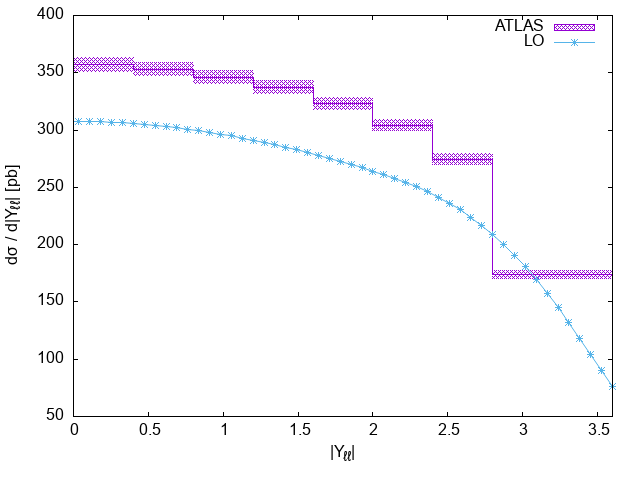
\includegraphics[width=.9\linewidth]{Yll.png}
\end{center}
We see that a similar offset as in the total cross section but it appears to be largely a normalization issue and the \emph{shape} itself is rather well described.

We can also have a look at the invariant-mass distribution (no ATLAS result for it in the paper).
\begin{center}
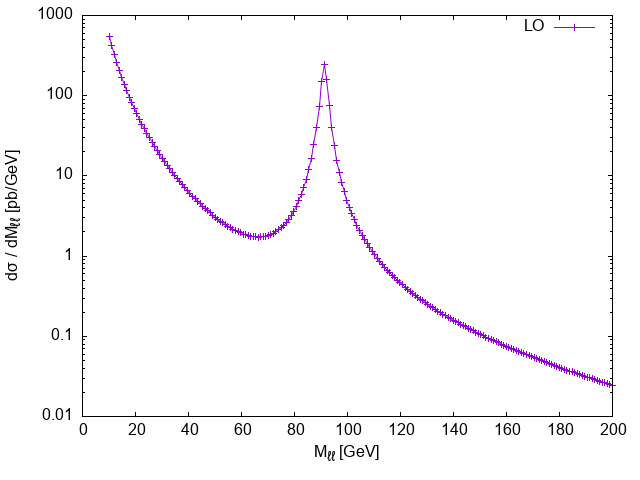
\includegraphics[width=.9\linewidth]{Mll.png}
\end{center}
We can see a similar picture of the photon pole and the Z-boson resonance as in the lepton collider example.
\end{document}